\documentclass[a4paper, 11pt]{article}
\usepackage[top=3cm, bottom=3cm, left=2.5cm, right=2.5cm]{geometry}
\usepackage{amsmath}
\usepackage{amsfonts}
\usepackage{graphicx}
\usepackage{psfrag}
\usepackage[utf8]{inputenc}
\usepackage[T1]{fontenc}
\usepackage[french]{babel}
\usepackage{hyperref}

\title{Document d'analyse : Factures}
\author{Pierre BONNEFOY, Ilyes ZEGHDALOU, Alexandre MARINE, Aloys LANA}


\begin{document}


\maketitle

\tableofcontents

\newpage
\section{Définition du Projet}
Projet qui analysera des factures. Nous allons nous cantonner à 2 types de messages :
\begin{itemize}
    \item L'Application Métier demandera le montant total de toutes les factures sur une période données et/ou par une entreprise spécifique.
    \item L'Application Métier demandera la liste des entreprises lui ayant vendu un produit spécifique.
\end{itemize}

\section{Modélisation de la Base de Données}
    \begin{center}
    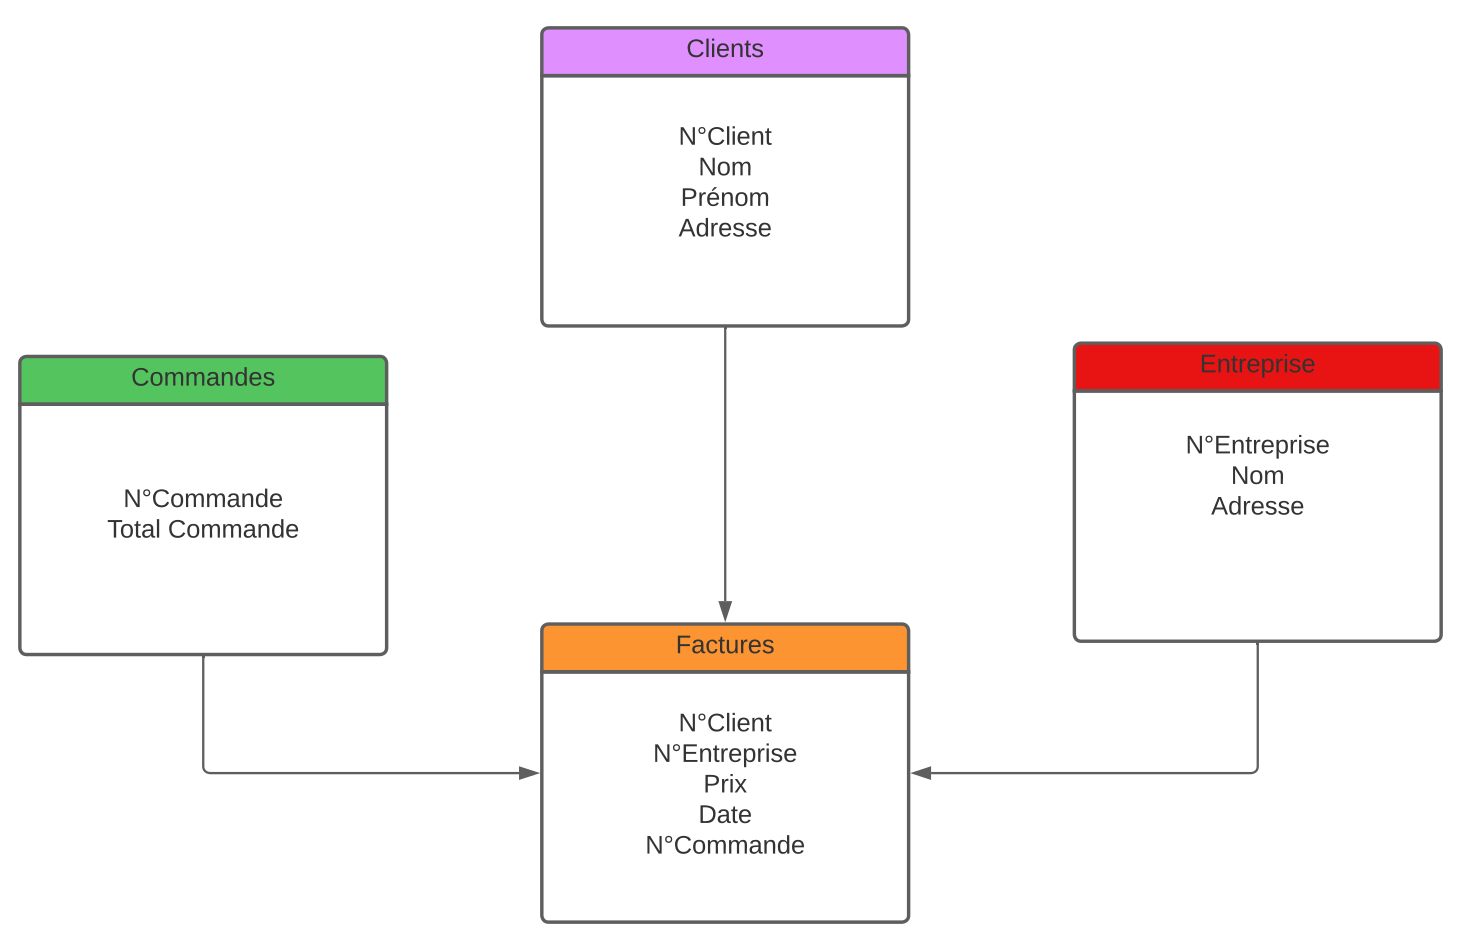
\includegraphics[scale=0.3]{schema_bdd.png}
    \end{center}

\section{Modélisations du Message 1}
    \subsection{Intitulé du Message}
        \subsubsection{Requête} 
        L'application métier demande à la Base de Données de lui envoyer le total de toutes les factures d'une entreprise cible et/ou d'une période cible.
        \subsubsection{Réponse}
        La Base de Données renvoie la somme de tous les totaux de chaque factures correspondant aux contraintes énoncées dans la requête.
    \subsection{Version JSON}
        \subsubsection{JSON Schéma}
        
        \subsubsection{JSON}

    \subsection{Version XML}
        \subsubsection{DTD}
        
        \subsubsection{XSD}
        
        \subsubsection{XML}

\section{Modélisations du Message 2}
    \subsection{Intitulé du Message}
        \subsubsection{Requête} 
        L'application métier demande à la Base de Données de lui envoyer la liste des entreprises lui ayant vendu un produit spécifique.
        \subsubsection{Réponse}
        La Base de Données renvoie la liste de toutes les entreprises lui ayant vendu ce produit.
    \subsection{Version JSON}
        \subsubsection{JSON Schéma}
            
        \subsubsection{JSON}
    
    \subsection{Version XML}
        \subsubsection{DTD}
            
        \subsubsection{XSD}
            
        \subsubsection{XML}

\section{Choix des Technologies}
Pour se projet nous allons utilisé du Python côté Serveur pour l'analyse et la gestion de la base de données. Pour le côté Application Métier, nous utiliserons les technologies Web (HTML, CSS et JavaScript). Nous utiliserons des messages écrits en JSON pour communiquer entre les deux dans un dossier qui simulera le réseau.

\section{Tâches et répartition}
    \subsection{Analyse de Fichiers}
    \begin{center}
    \begin{tabular}{|c|c|c|c|}
        \hline
        Enoncé de la Tâche & Personne assignée & Etat & Priorité\\
        \hline
        \hline
        Determiner les informations à relevé  & Pierre BONNEFOY & Finit & HAUTE \\
        \hline
        Repérage des Mots-Clés & Pierre BONNEFOY & Finit & HAUTE  \\
        \hline
        Développer une procédure de relevé & Pierre BONNEFOY & Finit & HAUTE  \\
        \hline
        Adaptation à plusieurs types de factures & Pierre BONNEFOY & En Cours & HAUTE  \\
        \hline
        Enregistrer dans la Base de Données & Pierre BONNEFOY & En Cours & HAUTE  \\
        \hline
    \end{tabular}
    \end{center}

    \subsection{Communication de la Base de Données}
    \begin{center}
    \begin{tabular}{|c|c|c|c|}
        \hline
        Enoncé de la Tâche & Personne assignée & Etat & Priorité\\
        \hline
        \hline
        Créer une Base de Données  & Alexandre MARINE & En Cours & HAUTE \\
        \hline
        Gérer l'accés a la Base de Données  & Alexandre MARINE & En Cours & HAUTE \\
        \hline
        Réception des requête de AM  & Alexandre MARINE & En Cours & HAUTE \\
        \hline
        Générer la réponse en JSON  & Alexandre MARINE & En Cours & HAUTE \\
        \hline
    \end{tabular}
    \end{center}

    \subsection{Génération des requêtes depuis l'application métier}
    \begin{center}
    \begin{tabular}{|c|c|c|c|}
        \hline
        Enoncé de la Tâche & Personne assignée & Etat & Priorité\\
        \hline
        \hline
        Générer les messages de réponse aux requêtes  & Alexandre MARINE & En Cours & HAUTE \\
        \hline
    \end{tabular}
    \end{center}

    \subsection{Réception des Réponses et Affichage coté Application Métier}
    \begin{center}
    \begin{tabular}{|c|c|c|c|}
        \hline
        Enoncé de la Tâche & Personne assignée & Etat & Priorité\\
        \hline
        \hline
        Scruter le Dossier de Simulation du réseau  & Aloys LANA & En Cours & HAUTE \\
        \hline
        Récuperer les données du fichier JSON  & Aloys LANA & Finit & HAUTE \\
        \hline
        Afficher les résultats  & Aloys LANA & En Cours & HAUTE \\
        \hline
        Supprimer les anciens messages  & Aloys LANA & En Cours & HAUTE \\
        \hline
    \end{tabular}
    \end{center}
\end{document}